\chapter{Data in Tao}
\label{c:data}
\index{Data|hyperbf}

The term \vn{``data''} denotes anything that can be calculated by
\tao. This includes the vertical orbit at a particular position or the
horizontal emittance of a storage ring. Data can be plotted or used in
lattice correction and design (\sref{c:opti}). This chapter explains
how data is organized in \tao while Section~\sref{s:init.data}
explains how to define the structures that hold the data in the
initialization files. When running \tao, the \vn{show data}
(\sref{s:show}) command can be used to view information about the
data.


%------------------------------------------------------------------------
\section{Data Organization}
\label{s:data.org}

\begin{figure}
  \centering
  \includegraphics[width=4in]{data-tree.eps}
  \caption[Data tree structure]
{A \vn{d2\_data} structure holds a set of \vn{d1\_data} structures. 
A \vn{d1\_data} structure holds an array of datums.}
  \label{f:data.tree}
\end{figure}

\index{d2_data}\index{d1_data}
The horizontal orbit at a particular BPM is an example of an
individual \vn{datum}.  For ease of manipulation, arrays of datums are
grouped into what is called a \vn{d1_data} structure. Furthermore,
sets of \vn{d1_data} structures are grouped into what is called a
\vn{d2_data} structure.  This is illustrated in
Figure~\ref{f:data.tree}.  For example, a \vn{d2_data} structure for
orbit data could contain two \vn{d1_data} structures --- one
\vn{d1_data} structure for the horizontal orbit data and another
\vn{d1_data} structure for the vertical orbit data. Each datum of,
say, the horizontal orbit \vn{d1_data} structure would then correspond
to the horizontal orbit at some point in the machine.

When issuing \tao commands, all the
data associated with a \vn{d2_data} structure is specified using the
\vn{d2_data} structure's \vn{name}.  The data associated with a
\vn{d1_data} structure is specified using the format
\begin{example}
  d2_name.d1_name
\end{example}
For example, if a \vn{d2_data} structure has the
name ``\vn{orbit}'', and one of its \vn{d1_data} structures has the
name ``\vn{x}'', then \tao commands that refer to the data in this
\vn{d1_data} structure use the name ``\vn{orbit.x}''. Sometimes there
is only one \vn{d1_data} structure for a given \vn{d2_data}
structure. In this case the data can be referred to simply by using
the \vn{d2_data} structure's name. The individual datums can be
referred to using the notation
\begin{example}
  <d2_name>.<d1_name>[<datum_index_range>]
\end{example}
For example, \vn{orbit.x[10]} refers to the horizontal orbit datum
with index 10. Notice that the beginning (lowest) datum index is user
selectable and is therefore not necessarily 1.

Ranges of data can be referred to using using a comma \vn{,} to
separate the indexes combined with the notation \vn{n1:n2} to specify
all the datums between \vn{n1} and \vn{n2} inclusive. For example
\begin{example}
  orbit.x[3:6,23]
\end{example}
refers to datums 3, 4, 5, 6, and 23. 

If multiple universes (\sref{s:universe}) are present, then the prefix \vn{"@"}
may be used to specify which universe the data applies to. The general notation is
\begin{example}
  [<universe_range>]@<d2_name>.<d1_name>[<datum_index>]
\end{example}
Commas and colons can be used in the syntax for \vn{<universe_range>}
like they are used in the syntax for \vn{datum_index_range}. When
there is only a single Universe specified, the brackets \vn{[} and
\vn{]} are optional. When not specified, the current ``viewed''
universe (\sref{s:view}) is assumed. The current \vn{viewed} universe
can also be specified using the number \vn{-1}. Examples:
\begin{example}
  [2:4,7]@orbit.x ! The \vn{orbit.x} data in universes 2, 3, 4 and 7.
  [2]@orbit.x     ! The \vn{orbit.x} data in universe 2. 
  2@orbit.x       ! Same as "2@orbit.x".
  orbit.x         ! The \vn{orbit.x} data in the current viewed universe.
  -1@orbit.x      ! Same as "orbit.x".
\end{example}

As explained in Section~\sref{s:data.anatomy}, each individual datum
has a number of components. The syntax to refer to a component is:
\begin{example}
  d2_name.d1_name[datum_index]|component
\end{example}
For example:
\begin{example}
  orbit.x[3:10]|meas     ! The measured data values
\end{example}

In referring to datums, a ``\vn{*}'' can be used as a wild card to 
denote ``all''. Thus:
\begin{example}
  *@orbit.x       ! The \vn{orbit.x} data in all universes.
  *               ! All the data in the currently viewed universe.
  *.*             ! Same as "*"
  *@*             ! All the data in all the universes. 
  *@*.*           ! Same as "*@*"
  orbit.x[*]|meas ! All measured values of orbit.x
  orbit.x[]|meas  ! No values. That is, the empty set.
  orbit.x|meas    ! Same as orbit.x[*]|meas.
\end{example}
The last example shows that when referring to an entire block of data
encompassed by a \vn{d1_data} structure, the \vn{[*]} can be omitted.


%------------------------------------------------------------------------
\section{Anatomy of a Datum}
\label{s:data.anatomy}

Each datum has a number of quantities associated with it:
\begin{example}
  ele_name       ! Character: Corresponding lattice element name.
  ele0_name      ! Character: Name of range marker element.
  data_type      ! Character: Type of data: "orbit.x", etc.
  merit_type     ! Character: Type of constraint: "target", "max", etc.
  data_source    ! Character: How the datum is calculated. "lattice", or "beam".
  ix_ele            ! Integer: Index of "ele" in the element list.
  ix_ele0           ! Integer: Index of "ele0" in the element list.
  ix_ele_merit      ! Integer: Lattice index where merit is evaluated.
  ix_d1             ! Integer: Index number in d1_data structure
  ix_data           ! Integer: Index in the global data array
  ix_dModel         ! Integer: Row number in the dModel_dVar derivative matrix.
  ix_bunch          ! Integer: Bunch number to get the data from.
  meas              ! Real: Measured datum value. 
  ref               ! Real: Measured datum value from the reference data set.
  model             ! Real: Datum value as calculated from the model.
  design            ! Real: What the datum value is in the design lattice.
  old               ! Real: The model at some previous time.
  base              ! Real: The value as calculated from the base model.
  fit               ! Real: The value as calculated from a fitting procedure.
  delta_merit       ! Real: Diff used to calculate the merit function term 
  weight            ! Real: Weight for the merit function term
  merit             ! Real: Merit function term value: weight * delta^2
  s                 ! Real: longitudinal position of ele.
  relative          ! Logical: Is this a relative datum?
  exists            ! Logical: Does the datum exist?
  good_model        ! Logical: Does the model component contain a valid value?
  good_meas         ! Logical: Does the meas component contain a valid value?
  good_ref          ! Logical: Does the ref component contain a valid value?
  good_user         ! Logical: Does the user want this datum used in optimization?
  good_opt          ! Logical: Can be used in Tao extensions.
  good_plot         ! Logical: Can be used in Tao extensions.
  useit_plot        ! Logical: Is this datum to be used in plotting?
  useit_opt         ! Logical: Is this datum to be used for optimization?
\end{example}
When running \tao, the \vn{show data}
(\sref{s:show}) command can be used to view the components of a datum. 
The \vn{set} command (\sref{s:set}) can be used to set some of these components.

%------------------------------------------------------------------------
\section{Datum values}
\label{s:datum.values}

\index{Data!measured}\index{Data!reference}\index{Data!model}
\index{Data!base}\index{Data!design}
A given datum has six values associated it:
\vspace{-2ex}
\begin{description}
  \vspace{-1ex}
  \item[meas] \Newline 
The value of the datum as obtained from some measurement. This is the
target or limit value that is used when running the optimizer. When
doing lattice design, the measured value corresponds to a constraint
value (\ref{c:opti}).
  \vspace{-1ex}
  \item[ref] \Newline
The reference datum value as obtained from some reference measurement. For example,
a measurement before some variable is varied could be designated as
the \vn{reference}, and the datum taken after the variation could be 
designated the \vn{measured} datum.
  \vspace{-0.5ex}
  \item[model] \Newline
The value of the datum as calculated from the \vn{model} lattice (\sref{s:lattice}).
  \vspace{-0.5ex}
  \item[design] \Newline
The value of the datum as calculated from the \vn{design} lattice (\sref{s:lattice}).
  \vspace{-0.5ex}
  \item[base] \Newline
The datum value as calculated from the \vn{base} lattice (\sref{s:lattice}).
  \vspace{-0.5ex}
  \item[old] \Newline
A datum value that was saved at some point in \tao's calculations. This value
can be ignored.
\end{description}

%------------------------------------------------------------------------
\section{Datums in Optimization}
\label{s:datum.opt}

When using optimization to do lattice correction or design
(\sref{c:opti}), Individual datums can be excluded from the process
using the \vn{veto} (\sref{s:veto}), \vn{restore} (\sref{s:restore}),
and \vn{use} (\sref{s:use}) commands. These set the \vn{good_user}
component of a datum. This, combined with the setting \vn{exists},
\vn{good_model}, \vn{good_meas}, \vn{good_ref}, and \vn{good_opt}
determine the setting of \vn{useit_opt} which is the component that
determines if the datum is used in the computation of the merit
function. The settings of everything but \vn{good_user} is determined
by \tao

\vn{exists} is set by \tao to True if the datum exists and False
otherwise. A datum may not exist if the type of datum requires the
designation of an associated element but the \vn{ele_name} component
is blank. For example, a \vn{d1_data} array set up to hold orbit data
may use a numbering scheme that fits the lattice so that , say, datum
number 34 in the array does not correspond to an existing BPM.

\vn{good_model} is set according to whether a datum value can be
computed from the \vn{model} lattice. For example, If a circular
lattice is unstable, the beta function and the closed orbit cannot be
computed.

\vn{good_meas} is set True if the \vn{meas} component value is set in
the data initialization file (\sref{s:init.data}) or is set using the
\vn{set} command (\sref{s:set}). Similarly, \vn{good_ref} is set True
if the \vn{ref} component has been set. \vn{good_ref} only affects the
setting of \vn{useit_opt} if the optimization is using reference data
as set by the global variable \vn{opt_with_ref} (\sref{s:globals}).

Finally \vn{good_opt} is meant for use in custom versions of \tao
(\sref{c:custom.tao}) and is always left True by the standard \tao code.

Example of using a \vn{show data} (\sref{s:show}) to check the logicals
in a datum:
\begin{example}
  Tao> show data 3@beta[1]

  Universe:   3
  %ele0_name         =
  %ele_name          = IP_L0
  %data_type         = beta.a
      ... etc ...
  %relative          =  F
  %exists            =  T
  %good_model        =  T
  %good_meas         =  F
  %good_ref          =  F
  %good_user         =  T
  %good_opt          =  T
  %good_plot         =  F
  %useit_plot        =  F
  %useit_opt         =  F
\end{example}
Here \vn{useit_opt} is False since \vn{good_meas} is False and
\vn{good_meas} is False since the \vn{meas} value of the datum (not
shown) was not set in the \tao initialization file.

%------------------------------------------------------------------------
\section{Tao Data Types}\index{Data!Data Types}
\label{s:data.types}

Data can be classified by how it is calculated. This is set by the
\vn{data_source} parameter associated with an attribute. If the data
comes from particle beam tracking, \vn{data_source} must be set to
\vn{"beam"}. For everything else, \vn{data_source} must be set to
\vn{"lattice"}. Some datum types, like the floor position of an
element, only make sense with a \vn{"lattice"} \vn{data_source}. Other
types, like \vn{dpx_dx}, only make sense with a \vn{"beam"}
\vn{data_source}. There is a third class of data types, like
\vn{emit.a} that can take a \vn{"lattice"} or \vn{"beam"}
\vn{data_source}. It is important to keep in mind that with this third
case, such datums will have a different value depending upon what
\vn{data_source} is used.  Table~\ref{t:data.beam} lists the
predefined data types in \tao that are valid for a \vn{"beam"}
\vn{data_source} (\sref{s:init.data}) and
Table~\ref{t:data.lattice} lists the predefined data types in
\tao that are valid for a \vn{"lattice"} \vn{data_source}.

\index{Data!Relative}
Associated with a datum are two lattice elements named
\vn{ele0_name} and \vn{ele_name}. Datums can be divided up into four
classes: \vn{Global} Datums, like the emittance in a circular
ring, do not have associated lattice elements and their corresponding
element names will be blank. Datums in the second class, like the beta
function at a given point, will only have one associated lattice
element given by \vn{ele_name} and \vn{ele0_name} will be blank.
Datums in the third class are associated with a section of the
lattice. For example, the maximum of the beta function in a lattice
region. In this case the \vn{ele0} element marks the beginning of the
region and \vn{ele} marks the end. The final class of datums, called
\vn{relative} datums, means that the datum value is set by the
difference between the value at the lattice element at \vn{ele0} and
the value at \vn{ele}. The betatron phase advance falls into this
category:
\begin{example}
  value = \(\phi\sb{x}\)(ele) - \(\phi\sb{x}\)(ele0)
\end{example}
If a relative datum has a blank \vn{ele0_name} then \vn{ele0} is taken
to be the beginning element of the lattice which is marker element
with index 0 named \vn{BEGINNING}.
The datum components \vn{ix_ele} and \vn{ix_ele0} are the index of
\vn{ele} and \vn{ele0} in the list of lattice elements.

For datums with \vni{non-relative} \vn{data_types} if there is also an
associated \vni{ele0} element then the \vn{model} value is dependent
upon the \vni{merit_type}. For example, with a \vn{beta.x}
\vn{data_type} the model value is determined by Table~\ref{t:eval2}
where \vn{i} goes from the \vn{ele} index to the \vn{ele0} index.
\begin{table}[ht]
\centering
{\tt
\begin{tabular}{|l|l|l|} \hline
  {\it Merit\_Type}       & {\it Model Value} \\ \hline 
  \vni{abs_max} & $\min |\beta_x(i)|$ \\ \hline 
  \vni{abs_min} & $\min |\beta_x(i)|$ \\ \hline 
  \vni{int_max} &                     \\ \hline
  \vni{int_min} &                     \\ \hline
  \vni{min}     & $\min \beta_x(i)$ \\ \hline 
  \vni{max}     & $\min \beta_x(i)$ \\ \hline 
  \vni{target}  & {\it Error}   \\ \hline 
\end{tabular}
}
\caption{\vn{Model} evaluation.}
\label{t:eval2}
\end{table}

\vn{wire} data simulates the measurement of a wire scanner. The angle specified
is the angle of the wire with respect to the horizontal axis. The measurement
then measures the second moment $<uu>$ along an axis which is 90 degrees off of
the wire axis. For example, \vn{wire.90} is a wire scanner oriented in the
vertical direction and measures the second moment of the beam along the
horizontal axis, $<xx>$. The resultant data is not the beam size, but the beam
size squared.

Emittance can be calculated in one of two ways. One way is to
calculate it from a tracked beam. The other is from the lattice using
the standard radiation integrals (see the Bmad manual). For a linear
lattice, the emittance varies along the length of the line while for a
circular lattice there is a single emittance number. \vn{emit.a}
and \vn{emit.b} are the standard normal mode emittances. With
beam tracking, there are also \vn{projected emittances} which give an
indication of what the beam looks like if projected onto the $x$ or
$y$ axes:
\begin{equation}
  \eta_x (\mbox{(projected)} = \sqrt{<x^2> <p_x^2> - <x p_x>^2}
\end{equation}
Notice that this does {\emph not} correspond to the standard emittance
definition in one dimension:
\begin{equation}
  \eta_x = \sqrt{<(x - \eta_x \, p_z)^2> <(p_x - \eta'_x \, p_z)^2> - 
  <(x - \eta_x \, p_z) \, (p_x - \eta'_x \, p_z)>^2}
\end{equation}
\vn{emit.x} and \vn{emit.y} are the projected emittances.
Also notice that the projected emittance is sometimes defined using
$x'$ and $y'$ in place of $p_x$ and $p_y$. However, in the vast
majority of cases, this does not appreciably affect the numeric
results.


\vn{beta.a} and \vn{beta.b} are the lattice beta functions. \vn{beta.x} and
\vn{beta.y} are beam projected beta functions defined by
\begin{equation}
  \beta.x = \frac{<x^{2}>}{\sqrt{<x^{2}> <x'^{2}> - <x x'>^{2}}}.
\end{equation}
where the average \vn{<>} is over all the particles in the beam.

The \vn{element_param.<param_name>} data type is for using lattice
element parameters. \vn{<param_name>} is the name of the
parameter. See the \bmad manual for the names associated with each
type of lattice element.  For example, the \vn{k1} quadrupole strength
would be given by:
\begin{example}
  element_param.k1
\end{example}

\vn{unstable_ring} is used for storage rings. The value of an
\vn{unstable_ring} datum is zero if the ring is stable and set to the
largest growth rate of all the normal modes of oscillation if the ring
is unstable. The value of an \vn{unstable_ring} datum is thus always
non-zero.  \vn{unstable_ring} is used in an optimization to avoid
unstable solutions (\sref{s:generalized.design}).

The \vn{expression:} data type allows the value of a datum to depend upon
the value of other datums or the value of variables. For example:
\begin{example}
  data_type = "expression: 1@beta.a[12]|model - 2@beta.a[12]|model"
\end{example}
With this, the value of the datum will be the difference between
\vn{beta.a[12]} for universe 1 and universe 2. To be valid, an
expression must be evaluated after it's components are evaluated. In
this example, the components are \vn{1@beta.a[12]|model} and
\vn{2@beta.a[12]|model}. Data evaluation is done universe by universe
starting with universe 1, then universe 2, etc. Within a given
universe, the order of evaluation can be complicated but in this case
a datum using an expression will always be evaluated after any datum
that appears earlier in the initialization file. In this example, the
datum should be in universe 2 or higher. Notice that while all datums
must be assigned a universe, in this case the value of the datum will
be independent of the universe it is in.


\index{Data!Calculation Method}
\index{unstable_ring}\index{beta}\index{alpha}\index{eta}\index{eta}
\index{etap}\index{phase}\index{orbit}\index{wire}\index{spin}
\index{cbar}\index{coupling}\index{floor}\index{r}\index{t}\index{tt}
\index{i5a_e6}\index{i5b_e6}\index{s_position}\index{e_tot}
\index{unstable_ring}\index{emittance}\index{chrom}\index{norm_emittance}
\index{sigma}\index{dpx_dx}\index{dpy_dy}\index{dpz_dz}\index{dpa_da}
\index{dpb_db}


\begin{table}[ht] 
\centering 
{\tt\small
\begin{tabular}{|l|l|l|} \hline

  beta.x, beta.y  beta.z      & Projected beta function            &          \\ \hline 
  beta.a, beta.b              & Normal-mode beta function          &          \\ \hline 

  dpx\_dx, dpx\_dy, etc.      & Bunch <x p\_x> / <$x^2$> \& Etc... &          \\ \hline 

  \begin{tabular}{@{}l}
    emit.x, emit.y, emit.z \\
    emit.a, emit.b, emit.c \\
  \end{tabular}               & Emittance                          & global   \\ \hline

  eta.x, eta.y                & Projected dispersion               &          \\ \hline 
  eta.a, eta.b                & Normal-Mode dispersion             &          \\ \hline 
  etap.x, etap.y              & Projected dispersion derivative    &          \\ \hline 
  etap.a, etap.b              & Normal-Mode dispersion derivative  &          \\ \hline 

  \begin{tabular}{@{}l}  
    norm\_emit.x, norm\_emit.x, norm\_emit.z \\ 
    norm\_emit.a, norm\_emit.b, norm\_emit.c 
  \end{tabular}               & Normalized beam emittance          &          \\ \hline 

  \begin{tabular}{@{}l}   
    sigma.x, sigma.y, sigma.z \\ 
    sigma.p\_x, sigma.p\_y, sigma.p\_z
  \end{tabular}               & Bunch size                         &          \\ \hline 

  spin.polarization, spin.theta, spin.phi
                              & Particle spin                      &          \\ \hline 

  wire.<angle>                & Wire scanner at wire angle <angle> &          \\ \hline


\end{tabular}
} 
\label{t:data.beam}
\caption{Predefined Data Types for \vn{"beam"} data\_source}
\end{table}

%----------------------------------------------------------------------------------------------

\begin{table}[ht] 
\centering 
{\tt\small
\begin{tabular}{|l|l|l|} \hline
  {\it Data\_Type}            & {\it Description}                  &          \\ \hline 

  alpha.a, alpha.b            & Normal-Mode alpha function         &          \\ \hline 
  beta.a, beta.b              & Normal-mode beta function          &          \\ \hline 
  bpm\_orbit.x, bpm\_orbit.y  & Measured orbit                     &          \\ \hline
  bpm\_phase.a, bpm\_phase.b  & Measured betatron phase            &          \\ \hline
  bpm\_eta.x, bpm\_eta.y      & Measured dispersion                &          \\ \hline

  \begin{tabular}{@{}l}
    bpm\_k.22a, bpm\_k.12a, \\
    bpm\_k.11b, bpm\_k12b
  \end{tabular}
                              & Measured coupling                  &          \\ \hline

  \begin{tabular}{@{}l}
    bpm\_cbar.22a, bpm\_cbar.12a, \\
    bpm\_cbar.11b, bpm\_cbar12b
  \end{tabular}
                              & Measured coupling                  &          \\ \hline

  cbar.11, cbar.12, cbar.21, cbar.22
                              & Coupling                           &          \\ \hline 

  \begin{tabular}{@{}l}
    chrom.a, chrom.b  \\
  \end{tabular}               & Chromaticity for a ring            & global   \\ \hline

  e\_tot                      & Beam total energy                  &          \\ \hline

  element\_param.<param\_name> & Lattice element parameter         &          \\ \hline

  \begin{tabular}{@{}l}
    emit.a, emit.b, emit.c \\
  \end{tabular}               & Emittance                          & global   \\ \hline

  eta.x, eta.y                & Projected dispersion               &          \\ \hline 
  eta.a, eta.b                & Normal-Mode dispersion             &          \\ \hline 
  etap.x, etap.y              & Projected dispersion derivative    &          \\ \hline 
  etap.a, etap.b              & Normal-Mode dispersion derivative  &          \\ \hline 

  expression: <arithmetic expression>
                              & See the text                       &          \\ \hline 

  floor.x, floor.y, floor.z, floor.theta 
                              & Global (``floor'') position        & relative \\ \hline 

  gamma.a, gamma.b            & Normal-mode gamma function         &          \\ \hline 

  i5a\_e6, i5b\_e6            & Normalized I5 radiation integral   &          \\ \hline

  k.11b, k.12a, k.12b, k.22a  & Coupling                           &          \\ \hline 
  momentum\_compaction        & Momentum compaction factor         & relative \\ \hline

  \begin{tabular}{@{}l}   
    multi\_turn\_orbit.x, multi\_turn\_orbit.p\_x \\ 
    multi\_turn\_orbit.y, multi\_turn\_orbit.p\_y \\
    multi\_turn\_orbit.z, multi\_turn\_orbit.p\_z \\
  \end{tabular}               & Bunch size                         &          \\ \hline 

  \begin{tabular}{@{}l}  
    norm\_emit.a, norm\_emit.b, norm\_emit.c 
  \end{tabular}               & Normalized beam emittance          &          \\ \hline 

  orbit.x, orbit.y            & Transverse orbit                   &          \\ \hline 
  orbit.p\_x, orbit.p\_y      & Transverse momenta                 &          \\ \hline 
  orbit.z, orbit.z\_p         & Longitudinal orbit and momenta     &          \\ \hline 
  orbit.amp\_a, orbit.amp\_b  & ``Invariant'' amplitude            &          \\ \hline 
  orbit.norm\_amp\_a, orbit.norm\_amp\_b  
                              & Energy normalized ``invariant'' amplitude &          \\ \hline 

  phase.a, phase.b            & Betatron phase                     & relative \\ \hline 

  phase\_frac.a, phase\_frac.b            
                              & \begin{tabular}{l}
                                  Fractional betatron phase \\       
                                  $-\pi < \phi_{\mbox{frac}} < \pi$ \\
                                \end{tabular}                      & relative \\ \hline 

  phase\_frac\_diff           & \begin{tabular}{l}
                                  Fractional betatron phase \\
                                  difference (a-b) $-\pi < d\phi_{\mbox{frac}} < \pi$
                                \end{tabular}                      & relative \\ \hline 

  r.$ij$                      & \begin{tabular}{l}
                                  Term in linear transfer map \\
                                  $1 \le i,j \le 6$
                                \end{tabular}                      & relative \\ \hline 

  s\_position                 & longitudinal length constraint     & relative \\ \hline 

  spin.polarization, spin.theta, spin.phi
                              & Particle spin                      &          \\ \hline 

  t.$ijk$                     & \begin{tabular}{l}
                                  Term in 2\Nd order transfer map \\
                                  $1 \le i,j,k \le 6$
                                \end{tabular}                      & relative \\ \hline 
  tt.$ijklm\ldots$            & \begin{tabular}{l}
                                  Term in n\Th order transfer map \\
                                  $1 \le i,j,k,\ldots \le 6$
                                \end{tabular}                      & relative \\ \hline 

  tune.a, tune.b              & Tune                               &          \\ \hline 
  unstable\_ring              & Nonzero if a ring is unstable      & global   \\ \hline

\end{tabular}
} 
\label{t:data.lattice}
\caption{Predefined Data Types for \vn{"lattice"} data\_source}
\end{table}

\vfill \break
{\vfill}
